\subsection{Stage 2 --- MD Elastic Evaluation}
\label{sec:stage2}

Each configuration is loaded into LAMMPS \citep{thompson2022} through its
Python API, and its elastic response is computed with a central-difference
strain protocol.

\paragraph{Multi-element MEAM build of LAMMPS.}
The stock LAMMPS distribution hard-codes the maximum number of MEAM species to
five, which is too few for the twelve-element library that Stage~4 produces. To
allow the multi-element runs this project needs, LAMMPS was rebuilt from source
with the species ceiling in the MEAM headers raised to 20, and the resulting
shared library was installed into the user environment so the Python API picks
it up automatically. Without this step the pipeline would stall on the first
composition with more than five distinct elements.

\paragraph{Elastic-property protocol.}
The procedure is:
\begin{enumerate}
	\item \textbf{Box construction.} A cubic supercell with a $\sim$4\,nm edge is
	      built from the dominant element's lattice structure and the
	      composition-weighted lattice parameter. Atom types are then reassigned
	      by \texttt{set type/fraction} to match the requested composition.
	\item \textbf{Relaxation.} An anisotropic pressure minimisation relaxes the
	      cell shape and the atomic positions together until the residual stress
	      is below a fixed tolerance.
	\item \textbf{Baseline stress.} The diagonal stress components
	      $\sigma_{xx}$, $\sigma_{yy}$, $\sigma_{zz}$ are recorded after a
	      \texttt{run~0}.
	\item \textbf{Strain protocol.} A strain $\delta=10^{-3}$ is applied along
	      each of $x,y,z$ in turn, positive and negative. The structure is
	      re-minimized at each strain and the stress tensor is recorded.
	\item \textbf{Elastic constants.} $C_{11}$ comes from the axial-stress
	      response and $C_{12}$ from the transverse response, by central
	      differences. This gives three independent $C_{11}$ samples and six
	      independent $C_{12}$ samples per simulation; the Voigt average
	      \citep{voigt} is the final estimate.
	\item \textbf{Engineering moduli.} Young's modulus and Poisson's ratio
	      follow from
	      \begin{equation}
	      	E = \frac{(C_{11}-C_{12})(C_{11}+2C_{12})}{C_{11}+C_{12}},
	      	\qquad
	      	\nu = \frac{C_{12}}{C_{11}+C_{12}}.
	      	\label{eq:elastic}
	      \end{equation}
\end{enumerate}

\paragraph{Physicality filter.}
A configuration is discarded, and removed from the configuration set, if any of
the following hold:
\begin{itemize}
	\item $E < 0$ (negative Young's modulus);
	\item $\nu < 0$ (negative Poisson's ratio);
	\item $\nu \geq 0.48$ (too close to the $(1-2\nu)=0$ singularity);
	\item $C_{11} < C_{12}$ (Cauchy/mechanical-stability violation).
\end{itemize}
The retained-corpus figure quoted in this report is the count that survives
this filter, not the number of configurations originally drawn. The same four
checks are enforced in the composition surrogate of Section~\ref{sec:comp_nn}
and in the Stage~5b optimizer of Section~\ref{sec:nnip}.

\paragraph{Why $(C_{11},C_{12})$ and not $(E,\nu)$ directly.}
Both surrogates in this project predict the two stiffness constants and recover
$(E,\nu)$ from Eq.~\eqref{eq:elastic} afterwards. The reason is that
$\nu = C_{12}/(C_{11}+C_{12})$ is ill-conditioned: for Mg- and Zn-rich
compositions $C_{11}$ and $C_{12}$ drift close together, the denominator
collapses, and a small error in either constant blows up the predicted $\nu$.
Regressing the raw constants keeps the targets on a well-behaved scale and
defers that division to the very end.

\paragraph{Parallel evaluation.}
The elastic-only batch path spreads configurations across worker processes,
one LAMMPS instance per physical core. On a 4-core (8-thread) host this runs
about three to four times faster than the sequential path.

The protocol was executed on the full retained corpus, and the resulting
$(E,\nu)$ and $(C_{11},C_{12})$ values are stored with each composition in a
shared elastic-property database. Across the set, $E$ runs from a few GPa to
nearly 400\,GPa. The dataset-level statistics over the $7815$ filtered
configurations are listed in Table~\ref{tab:md_stats}, and the distributions
are plotted in Figure~\ref{fig:md_dist}. Figure~\ref{fig:md_scatter} colours
the $E$--$\nu$ scatter by the dominant element of each composition.

% AUTO-GENERATED by src/stats/ -- do not edit by hand
\begin{table}[htbp]
\centering
\caption{Summary statistics of the LAMMPS-evaluated elastic properties over the physicality-filtered dataset ($0<E<400$\,GPa, $0<\nu<0.5$). Auto-generated from 7879 configuration records.}
\label{tab:md_stats}
\begin{tabular}{lrrrrrr}
\hline
 Quantity   &    N &    Mean &   Median &   Std. &   Min &     Max \\
\hline
 $E$ (GPa)  & 7815 & 132.877 &  103.610 & 69.098 & 3.070 & 398.310 \\
 $\nu$      & 7815 &   0.319 &    0.326 &  0.063 & 0.011 &   0.497 \\
\hline
\end{tabular}
\end{table}


\begin{figure}[h]
	\centering
	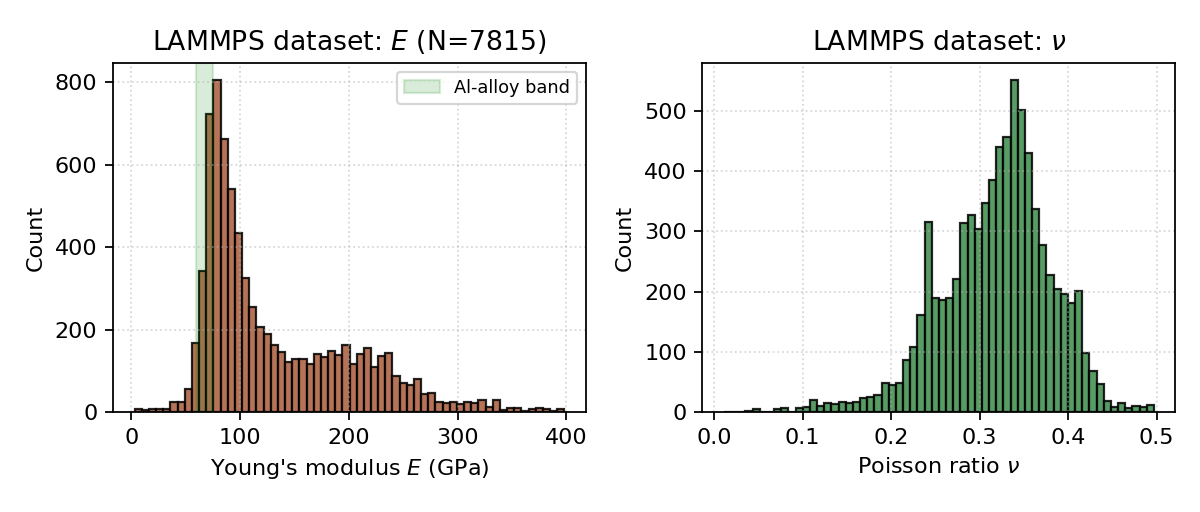
\includegraphics[width=0.95\textwidth]{figures/dataset_distributions.png}
	\caption{Histograms of $E$ (left) and $\nu$ (right) over the
	LAMMPS-evaluated dataset. The shaded band on the left panel marks the
	experimentally expected 60--75\,GPa range for aluminium alloys, which
	contains $14.0\,\%$ of the physical sample.}
	\label{fig:md_dist}
\end{figure}

\begin{figure}[h]
	\centering
	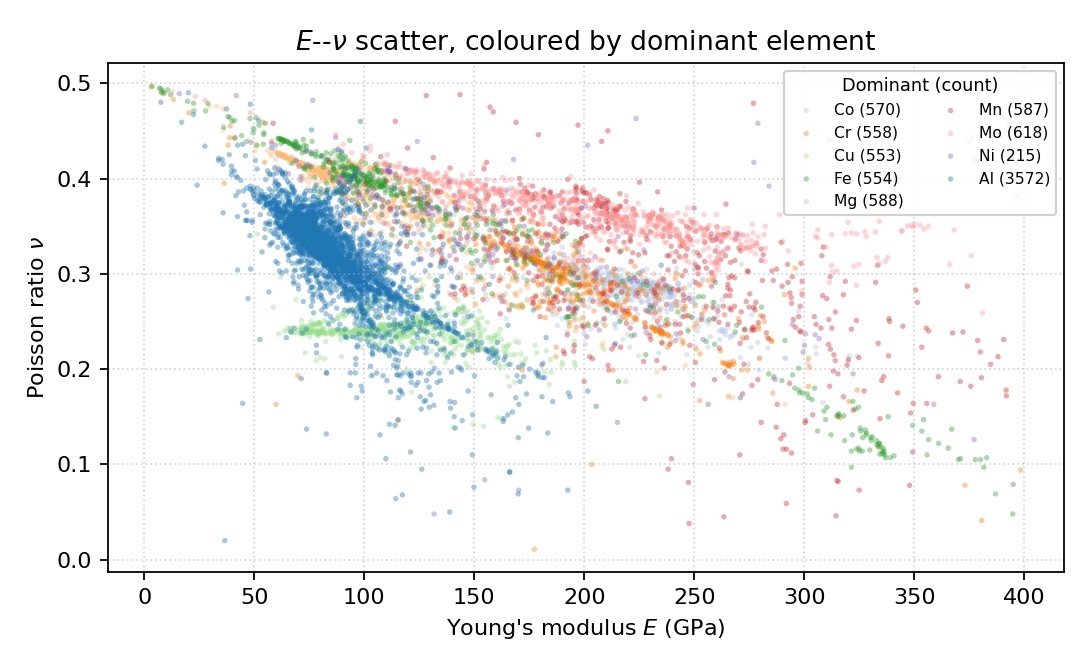
\includegraphics[width=0.78\textwidth]{figures/E_nu_scatter.png}
	\caption{$E$--$\nu$ scatter of the LAMMPS-evaluated dataset, coloured by
	the dominant element. The Al-dominant cloud sits in the expected
	60--75\,GPa band; refractory-rich (Mo, Cr, Fe) compositions populate the
	high-$E$ wing, while Mg- and Zn-rich points push $\nu$ towards $0.5$.}
	\label{fig:md_scatter}
\end{figure}
